%! TEX program = pdflatex
% =====================================================================
% Journal of Conflict Resolution (SAGE) submission, Research Article.
% This file is a journal-ready draft built on the shared master content
% in ../../content/. To swap in the SAGE class file:
%
%   1. Download sagej.cls + SageH.bst from
%      https://uk.sagepub.com/en-gb/eur/manuscript-submission-guidelines
%   2. Replace the preamble below with \documentclass[Crown,times]{sagej}
%      following the SAGE skeleton; the \input{...} bodies and
%      \bibliography{...} below remain unchanged.
%
% Until then this file produces a single-column double-spaced draft
% that matches JCR / SAGE submission requirements (one-column,
% Harvard-style author-year citations, blinded title page).
% =====================================================================
\documentclass[12pt,a4paper]{article}

\usepackage[utf8]{inputenc}
\usepackage[T1]{fontenc}
\usepackage{lmodern}
\usepackage[margin=1in]{geometry}
\usepackage{setspace}
\onehalfspacing
\usepackage{amsmath,amssymb,amsthm,mathtools}
\usepackage{booktabs,multirow,array,tabularx}
\usepackage{graphicx}
\usepackage[hidelinks,colorlinks=false]{hyperref}
\usepackage{enumitem}
\usepackage{xcolor}
\usepackage{microtype}
\usepackage{caption}
\usepackage{subcaption}
\usepackage{tikz}
\usetikzlibrary{calc,arrows.meta,decorations.pathreplacing,positioning,fit,backgrounds}
\usepackage[round,authoryear,sort&compress]{natbib}
\bibliographystyle{plainnat}
\captionsetup{font=small,labelfont=bf,labelsep=period,justification=justified}
\setlist{itemsep=2pt,topsep=3pt,parsep=0pt}
\graphicspath{{../../figures/}}

\theoremstyle{plain}
\newtheorem{theorem}{Theorem}[section]
\newtheorem{proposition}[theorem]{Proposition}
\newtheorem{lemma}[theorem]{Lemma}
\newtheorem{corollary}[theorem]{Corollary}
\theoremstyle{definition}
\newtheorem{definition}[theorem]{Definition}
\newtheorem{assumption}[theorem]{Assumption}
\theoremstyle{remark}
\newtheorem*{remark}{Remark}

\newcommand{\R}{\mathbb{R}}
\newcommand{\E}{\mathbb{E}}
\renewcommand{\Pr}{\mathbb{P}}
\newcommand{\Ind}{\mathbf{1}}
\DeclareMathOperator*{\argmin}{arg\,min}
\DeclareMathOperator*{\argmax}{arg\,max}

\title{\textbf{Bounds and Estimators for the Civilian-to-Combatant Death Ratio\\ from Aggregation of Conflicting Sources}}
% NOTE: JCR uses double-blind review. For peer review submission, comment out
% the \author{} block below and replace with \author{Anonymous}; restore for
% the camera-ready / accepted version. The detached title page lives in
% ../../submissions/jcr/title_page.tex (also produced for SAGE upload).
\author{%
  David H.\ Silver\thanks{Independent researcher, Poughkeepsie, NY 12603, USA. Email: \href{mailto:silverdavi@gmail.com}{\texttt{silverdavi@gmail.com}}. ORCID: \href{https://orcid.org/0000-0002-3071-304X}{0000-0002-3071-304X}.}\\
  \small Independent researcher\\
  \small Poughkeepsie, NY, USA\\[2pt]
  \small\emph{Submitted to Journal of Conflict Resolution, Research Article}}
\date{\today}

\begin{document}
\maketitle

\begin{abstract}
% Master abstract. Journal-specific main files override or wrap this.
\noindent
Casualty figures in armed conflict are reported by sources with opposing incentives: belligerents inflate enemy combatants killed and deflate civilians; advocacy and intergovernmental bodies push the other way. We treat the civilian-to-combatant death ratio as a partially identified parameter and ask what its value can be when conflicting sources are aggregated. The paper delivers two objects.

\textbf{(1) Bounds from under-fudgible relations.} Under a one-parameter model in which civilian adult men face $\mu$ times the death rate of women and children, we give a sharp identified set for the combatant share $q=D_M/D$ as a function of population structure, the demographic composition of the dead, and pre-war combatant stock; intersected with the manpower bound $D_M\le M$, this is a closed-form interval. Because the inputs are measured by different, non-aligned institutions, the relation is under-fudgible: moving any one input to rescue a disputed claim forces a compensating, visible move in an independently measured quantity. We define the \emph{contradiction radius} $\rho$ of a claim---the smallest standardised revision of a single independent input that makes it feasible---turning ``we dispute your number'' into ``name which measurement is wrong, and by how much.''

\textbf{(2) Sensitivity bands under political bias.} Each source is allowed to be Huber $\varepsilon_i$-contaminated; the analyst's political-bias prior on a source enters as $\varepsilon_i$. We give a closed-form first-order sensitivity band that absorbs the assumed contamination, a patternwise worst-case envelope, and a quantile-displacement bound under an explicit posterior-weight condition.

In the Gaza 2023--2026 application---anchored on the Ministry of Health demographic record, whose composition is consistent with an independent household survey---the identified set for $q$ is $[0,\nQOneRound{}\%]$ under only the weak assumption that civilian men are at least as exposed as women and children ($\mu\ge 1$), and $[0,\nQTwoRound{}\%]$ under exposure ratios informed by historical conflicts with known combatant status ($\mu\in[2,3.5]$). The public Israel Defense Forces figure of $17$--$25$k combatants killed converts to $q\approx \nIdfQLoRound{}$--$\nIdfQHiRound{}\%$ over the recorded toll. Its upper end is arithmetically infeasible: no exposure ratio $\mu\ge 1$ admits it, at a contradiction radius of $\nRhoOmegaAgRound{}$--$\nRhoOhchrCalRound{}$ times the conservative uncertainty scale attached to the demographic record. Its lower end ($q\approx \nIdfQLoRound{}\%$) sits at the very edge of the $\mu\ge 1$ set---attainable only if civilian men died at essentially the same rate as women and children ($\mu\le \nMuIdfLo{}$)---and leaves the set beyond that point, at a radius of $\nRhoIdfLoCalRound{}$ such units against the historically informed range. The rejection under calibrated exposure survives an upward correction of the death toll and, separately, a $5\%$ contamination allowance on each core input in the paper's first-order sensitivity band. Independent evidence---demographic decompositions, the military's own leaked internal database of named militant dead, and a fully documented spatial Bayesian model---concentrates well below the claim, at civilian-to-combatant ratios of roughly $\nCcrAtQOne{}{:}1$ to $\nSpatialCcr{}{:}1$ on direct deaths. The framework is symmetric: it tests the polar claim of zero combatant deaths the same way; that claim survives the demographic test and is rejected on documentary grounds.


\bigskip
\noindent\textbf{Keywords:} casualty estimation; civilian victimisation; partial identification; robust Bayesian inference; source aggregation; Gaza; under-fudgible relations.
\end{abstract}

\section{Introduction}

\subsection{The aggregation problem}

Casualty figures in armed conflict are reported by sources with opposing incentives. Belligerents inflate enemy combatants killed and deflate civilians; advocacy organisations, opposing belligerents, and intergovernmental bodies have symmetric incentives in the other direction. Naive aggregation is therefore biased in a direction that depends on which side the analyst trusts more. The tempting conclusion is that civilian-to-combatant ratios are too politicised to analyse statistically.

We argue for a narrower position. Conflicting source aggregates fail in well-understood ways, but the parameters they purport to measure are jointly constrained by a small number of relations whose inputs are measured by different, non-aligned institutions. An analyst who treats every belligerent source as adversarial can still recover an informative bound by exploiting these constraints; what cannot be recovered without further assumptions is the position of the truth \emph{within} the bound. This separation---bounds from data, position from politics---is the organising principle of the paper. The framework is a \emph{diagnostic}, not an oracle: its purpose is to force any dispute about a casualty claim to name the specific independent measurement being contested, and to quantify how far that measurement would have to be wrong.

\paragraph{A worked example.} Suppose a population is $73\%$ women and children ($w=0.733$) and records of the dead show that $56\%$ of $70{,}000$ dead are women and children ($\omega=0.560$). If violence were blind to demographics, the dead would mirror the population, so the deficit of women and children among the dead is informative: some of the dead were combatants (all adult men, by assumption), and possibly civilian adult men were more exposed than their population share suggests. If civilian men and women die at \emph{equal} per-capita rates, arithmetic (Section~\ref{sec:bounds}) turns these three numbers into a combatant share of $q\approx 25\%$. If civilian adult men die at \emph{twice} the rate of women and children---the kind of differential found when the same method is calibrated on historical conflicts where the answer is known \citep{frost2026}---the same arithmetic gives $q\approx 6\%$. The interval $[{\sim}6\%,{\sim}25\%]$ is what the data alone deliver; a claimed $q$ of $30\%$ is outside it for \emph{every} admissible exposure ratio and can only be rescued by asserting that the census or the death records are wrong, by an amount the framework computes in standard-error units. That amount is the claim's \emph{contradiction radius}.

The closest precedents are \citet{spagat2009} on the contestation of war-death estimates, \citet{lumpricebanks2013} on multiple systems estimation under reporting failure, \citet{radford2023} on Bayesian inference of conflict losses with reporting biases, \citet{vesco2026} on probabilistic UCDP underreporting, and \citet{gomez2025} on uncertainty quantification for Gaza mortality. Methodologically we draw on partial identification \citep{manski2003,manski2007,molinari2020,klinetamer2023} and robust Bayesian analysis \citep{huber1964,huber1981,berger1986}. On Gaza specifically, complementary demographic decompositions of the identified dead have been developed by \citet{cockerill2024} and \citet{frost2026}, and we engage with both.

\subsection{Two deliverables}

\paragraph{Bounds.} Where can the civilian-to-combatant ratio possibly lie, given a set of independently measured demographic and manpower facts? The answer is a sharp identified set in the sense of Manski's partial-identification programme \citep{manski2003,tamer2010,romanoshaikh2010}. If the identified set is narrow, no source-aggregation rule can pull the truth outside it. The width is determined by the data, not by the analyst's politics.

\paragraph{Confidence coefficients.} How much can the analyst's political-bias prior on each source widen this set? Each source is Huber $\varepsilon$-contaminated \citep{huber1981,berger1986}: it is true with probability $1-\varepsilon$ and adversarial with probability $\varepsilon$. A bias-robust sensitivity band inflates the face-value interval by $\sum_i\varepsilon_i R_i$ to first order in $\varepsilon$, where $R_i$ is the diameter of the identified set when source $i$ is removed; conditional on a realised contamination of source $i$, the worst-case displacement is $R_i$ itself. Setting $\varepsilon_i\approx 1$ for belligerent claims and $\varepsilon_i\approx 0.05$ for census-grade sources gives an interval honest about which inputs are doing the work.

The two objects are complementary: the first is information that survives any reasonable politics; the second is the rate at which uncertainty grows as the analyst dials in distrust of specific sources.

\subsection{The under-fudgible mechanism}

The bounds are not vacuous because of demographic arithmetic. Consider any claimed decomposition of the dead into combatants and civilians. The claim must simultaneously respect (i) the demographic composition of the identified dead, (ii) the demographic composition of the pre-war population, (iii) the size of the armed group's pre-war stock, and (iv) the plausible range of the civilian adult-male exposure differential. These quantities are measured by \emph{different} institutions: a national or UN census produces (ii); a health ministry, the OHCHR, or a household survey produces (i); independent military-balance assessments produce (iii); and (iv) can be calibrated on historical conflicts where combatant status was recorded \citep{frost2026}. They are not equally manipulable, and---critically---they cannot all be moved at once without the moves being visible.

We call a relation between conflict statistics \emph{under-fudgible} when its inputs are reported by non-aligned institutions (or have uncontroversial physical bounds), so that adjusting any single input to rescue a disputed claim forces a measurable deviation in at least one independently measured quantity. This is a heuristic property of a measurement system, not a formal axiom; what is formal is its consequence, the contradiction radius of Section~\ref{sec:contradiction}, which quantifies exactly how large the forced deviation is for any specific claim. The trigger is \emph{joint inconsistency}, not the size of the claim: the same machinery rejects a claimed combatant share that is too high and one that is too low, against the same feasible set. This symmetry matters. The diagnostic responds to the demographic content of a claim, not to its political direction, and Section~\ref{sec:gaza} applies it in both directions.

\subsection{Contributions and roadmap}

The paper delivers, in order of importance:

\begin{enumerate}[leftmargin=*,label=(\roman*)]
\item \emph{A sharp identified set} for the combatant share $q=D_M/D$ under bounded differential exposure of civilian adult men, intersected with the manpower bound $D_M \le M$ (Section~\ref{sec:bounds}). The set is a closed-form interval computable from four numbers.
\item \emph{The contradiction radius} $\rho$: a feasibility test for any disputed claim, stated as a distance-to-feasibility optimisation in standard-error units (Section~\ref{sec:contradiction}). It converts ``we dispute your number'' into ``name which independent input is wrong, and by how many standard errors.''
\item \emph{A bias-robust sensitivity band} under Huber $\varepsilon$-contamination of each source: a patternwise worst-case envelope, a first-order band for the interval endpoints, and a quantile-displacement bound under an explicit posterior-weight condition (Section~\ref{sec:bias}).
\item \emph{A precision-weighted aggregation rule} for multiple demographic sources, with an explicit caveat for selection-biased sources (Section~\ref{sec:aggregation}).
\item \emph{A Gaza 2023--2026 application} (Section~\ref{sec:gaza}): the identified set, the contradiction radius of the public IDF combatant-death claim under every anchor and exposure assumption, a sensitivity grid over all contested inputs, and a comparison against every independent method known to us---which all reject the claim while disagreeing only within the identified set. A fully documented spatial Bayesian model (Appendix~\ref{app:spatial}) illustrates where a specific set of modelling assumptions lands \emph{within} the set.
\item \emph{An 81-conflict overview} (Section~\ref{sec:empirical}) mapping where the diagnostic can and cannot be applied sharply, with per-conflict tables in the supplement.
\end{enumerate}

Proofs are collected in Appendix~\ref{app:proofs}. The method does not assign moral responsibility, estimate indirect deaths, or replace forensic work.

\section{Setup}\label{sec:setup}

A conflict produces $D\in\mathbb N$ deaths in $[t_0,t_1]$ in a population of size $N$. Each death is a combatant ($C=1$) or civilian ($C=0$); write $D_M=\sum_i\Ind\{C_i{=}1\}$, $D_C=D-D_M$, and the targets
\[
q = D_M / D \in [0, 1], \qquad r = D_C / D_M = (1 - q)/q.
\]
Each death has a demographic class $k\in\mathcal K=\{\text{child},\text{adult-female},\text{adult-male}\}$. To keep the two central quantities visually distinct we reserve the \emph{Latin} letter $w$ for the population and the \emph{Greek} letter $\omega$ for the dead:
\begin{align*}
w \;&=\; \text{women-and-children share of the \underline{population}},\\
\omega \;&=\; \text{women-and-children share of the \underline{dead}}.
\end{align*}
Formally, $\omega_k=D_k/D$ is the share of class $k$ among the dead and $p_k$ its share in the population; $\mathrm{AM}$ denotes adult males (18 and over), with population share $a=p_{\mathrm{AM}}=1-w$; $\omega=\sum_{k\ne\mathrm{AM}}\omega_k$. Let $M$ be the pre-war combatant stock and $f=M/N$. We take combatants to be in $\mathrm{AM}$; female and minor combatants enter as a small slack $\bar\eta\le 0.03$ (Remark~\ref{rem:female-combatants}).

\begin{table}[ht]
\centering
\caption{\textbf{Core notation and measurement channels.} The distinction between $w$ (population) and $\omega$ (dead) is load-bearing throughout: $w$ comes from a census taken before or independently of the fighting, $\omega$ from records of the dead.}
\label{tab:notation}
\begin{small}
\begin{tabularx}{\textwidth}{@{}lll>{\raggedright\arraybackslash}X@{}}
\toprule
Symbol & Meaning & Role & Typical source \\
\midrule
$D$              & total deaths in window      & input    & ministry of health, OCHA, UCDP, survey \\
$D_M, D_C$       & combatant, civilian deaths  & target   & decomposition of $D$ \\
$q=D_M/D$        & combatant share of dead     & estimand & --- \\
$w$              & women+children share \emph{of population} & input & census, UN Population Division \\
$a=1-w$          & adult-male (18$+$) share \emph{of population} & input & census / age pyramid \\
$\omega$         & women+children share \emph{of the dead} & input   & identified-deaths records (e.g.\ MoH) \\
$M$              & combatant stock at $t_0$    & input    & IISS / RUSI / CSIS / intelligence \\
$[\mu_{\mathrm{lo}},\mu_{\mathrm{hi}}]$ & admissible exposure-ratio range & assumption & calibrated from historical conflicts \\
$\rho$           & contradiction radius of a claim  & output   & SE-units to feasibility; see \S\ref{sec:contradiction} \\
\bottomrule
\end{tabularx}
\end{small}
\end{table}

The last row anticipates the paper's diagnostic. The \emph{contradiction radius} $\rho$ of a disputed claim is the smallest number of measured standard errors by which at least one independent input ($\omega$, $w$, or $M$) would have to move for the claim to become consistent with all the others; $\rho=0$ means consistent, $\rho=3$ means some independently measured quantity must be wrong by three standard errors, and values in the double digits mean the claim requires an input to be wrong by an amount that measurement error cannot plausibly produce. Section~\ref{sec:contradiction} makes this precise.

\paragraph{Sources.} We use five channels: an independent population census $(p_k,N)$; demographic records of the dead returning sample shares $\hat\omega_k$; aggregate death totals $\hat D$; belligerent combatant-death claims $\hat D_M$; and independent manpower estimates $\hat M$. Each source $i$ is allowed to be $\varepsilon_i$-contaminated in Huber's sense \citep{huber1964,berger1986}: it draws from the truth with probability $1-\varepsilon_i$ and from an arbitrary adversary with probability $\varepsilon_i$.

\subsection{Source aggregation}\label{sec:aggregation}

When several independent sources $i=1,\dots,m$ report the same scalar parameter $\theta$ with reported point estimates $\hat\theta_i$ and standard errors $\hat\sigma_i$, the natural \emph{precision-weighted} aggregate is
\begin{equation}\label{eq:agg}
\hat\theta_{\mathrm{agg}} \;=\; \frac{\sum_i\hat\theta_i/\hat\sigma_i^2}{\sum_i 1/\hat\sigma_i^2},
\qquad
\hat\sigma_{\mathrm{agg}}^2 \;=\; \Bigl(\sum_i 1/\hat\sigma_i^2\Bigr)^{-1}.
\end{equation}

\begin{proposition}[Aggregation under conflicting sources]\label{prop:agg}
If sources are independent and unbiased, with variances treated as known (with estimated $\hat\sigma_i^2$ the statement holds conditionally on the variance estimates and asymptotically), $\hat\theta_{\mathrm{agg}}$ in \eqref{eq:agg} is the minimum-variance unbiased linear estimator of $\theta$. If source $i$ has bias $b_i$, the aggregate has bias $\bigl(\sum_i b_i/\hat\sigma_i^2\bigr)/\bigl(\sum_i 1/\hat\sigma_i^2\bigr)$. Allowing $\varepsilon_i$-contamination (Section~\ref{sec:bias}) in which the contaminated report is displaced from the truth by at most $R_i$, the worst-case bias of $\hat\theta_{\mathrm{agg}}$ is at most $\sum_i\varepsilon_i R_i\cdot \hat\sigma_{\mathrm{agg}}^2/\hat\sigma_i^2$.
\end{proposition}
Proof in Appendix~\ref{app:proofs}.

Precision weighting presupposes that the sources measure the \emph{same} estimand. When one source is subject to a known selection mechanism---as with the OHCHR verification sample in the Gaza application, which is heavily weighted toward residential-strike deaths \citep{spagatcockerill2024}---the honest treatment is not to blend it into the aggregate but to use it as a stratum-specific measurement and anchor the analysis on the source whose selection is best understood. Section~\ref{sec:gaza} applies this rule: the Ministry of Health record, whose demographic composition is corroborated by an independent household survey \citep{spagatlgh2026}, is the primary anchor, and results are reported for the alternative anchors so the reader can see exactly how anchor choice propagates.

\section{Bounds: partial identification of \texorpdfstring{$q$}{q}}\label{sec:bounds}

This section delivers a sharp identified set for $q$ that any source-aggregation rule must respect. We begin with a benchmark assumption, then weaken it. Proofs are in Appendix~\ref{app:proofs}.

\begin{assumption}[Exchangeable collateral]\label{ass:ec}
Civilians of all demographic classes face equal per-capita death hazard.
\end{assumption}

Under Assumption~\ref{ass:ec} the combatant share is point-identified by a single rearrangement: civilian deaths split between the women-and-children class and the adult-male class in proportion to their civilian population shares, so
\begin{equation}\label{eq:ident}
q = 1 - \frac{\omega(1 - f)}{w}.
\end{equation}
The intuition is direct: $\omega$ falls short of the population share $w$ only to the extent that deaths are diverted to the (all-male) combatant pool.

\begin{remark}\label{rem:female-combatants}
Suppose a fraction $\eta\le\bar\eta=0.03$ of combatant \emph{deaths} is recorded in class $W$. This is a classification slack: the combatant stock itself stays in $\mathrm{AM}$, so the civilian split $S=w/(w+\mu(a-f))$ is unchanged. The identity becomes $\omega=(1-q)S+\eta q$, the true share is $q_{\mathrm{true}}=(S-\omega)/(S-\eta)$, and the no-slack value $q_{\eta=0}=(S-\omega)/S$ understates it by exactly
\[
q_{\mathrm{true}}-q_{\eta=0}\;=\;\frac{\eta\,q_{\mathrm{true}}}{S}\;=\;\frac{\eta\,q_{\eta=0}}{S-\eta}\;\ge\;0
\qquad(S>\eta,\ q_{\mathrm{true}}\ge 0).
\]
At the values in Section~\ref{sec:gaza}, where $S>\bar\eta$ throughout ($S\ge 0.597$ for $\mu\le 2$) and $q_{\eta=0}\le 0.26$, a loose uniform bound over $\mu\in[1,2]$ is $\bar\eta\cdot 0.26/(0.597-\bar\eta)\approx 1.4$ percentage points; the exact understatement is smaller and falls with $\mu$ ($1.05$ points at $\mu=1$, $0.33$ at $\mu=2$), since $q_{\eta=0}$ shrinks faster than $S$. Readers who want this slack should widen the \emph{upper} endpoints below by $\bar\eta\, q_{\eta=0}/(S-\bar\eta)$; we otherwise suppress it.
\end{remark}

Assumption~\ref{ass:ec} is strong: civilian adult men typically face higher per-capita exposure than women and children due to outside work, food queues, rescue activity, and circumstantial proximity to combat. We weaken it to a one-parameter family.

\begin{assumption}[$\mu$-bounded differential exposure]\label{ass:mu}
There exists $\mu\in[\mu_{\mathrm{lo}},\mu_{\mathrm{hi}}]$ such that, conditional on being civilian, class $\mathrm{AM}$ has per-capita death rate $\mu$ times that of class $W$.
\end{assumption}

\begin{theorem}[Sharp identified set]\label{thm:bounds}
Suppose $f\le a$ and Assumption~\ref{ass:mu} holds. Given $(\omega,w,a,f)$ and the exposure range $[\mu_{\mathrm{lo}},\mu_{\mathrm{hi}}]$, the identified set for $q$ is the image of the monotone-decreasing curve
\begin{equation}\label{eq:qmu}
q(\mu) = 1 - \omega\,\frac{w+\mu(a-f)}{w}, \qquad \mu\in[\mu_{\mathrm{lo}},\mu_{\mathrm{hi}}],
\end{equation}
giving the sharp interval $[q(\mu_{\mathrm{hi}}),\,q(\mu_{\mathrm{lo}})]\cap[0,1]$.
\end{theorem}

\begin{corollary}[Manpower bound]\label{cor:popbudget}
$q\le M/D$, so whenever the endpoints below are ordered, the joint feasible interval is
\[
q \in \bigl[\max\{0,\,q(\mu_{\mathrm{hi}})\},\; \min\{1,\,q(\mu_{\mathrm{lo}}),\,M/D\}\bigr];
\]
if the lower endpoint exceeds the upper the set is empty and the inputs are jointly infeasible---the event detected by a positive contradiction radius in Section~\ref{sec:contradiction}.
\end{corollary}

\paragraph{Calibrating the exposure range.} The exposure ratio $\mu$ is the framework's only behavioural parameter, and it can be disciplined empirically rather than stipulated. \citet{frost2026} identifies the civilian male exposure differential from the male-to-female death ratio just \emph{above} the combatant age range---where the combatant share is mechanically near zero---and validates the procedure on historical Gaza conflicts recorded by B'tselem, where combatant status is known: there, the observed male-to-female ratio at the top of the combatant age band is $3.4{:}1$ while the effective differential through the combatant ages is $5{:}1$, so the observable ratio is itself a conservative lower bound. Airstrike-specific data suggest smaller differentials ($\approx 1.3$; \citealp{cockerill2024}), consistent with indiscriminate mechanisms; ground operations push the differential up. We therefore report the identified set on a grid $\mu\in\{1, 1.5, 2, 2.5, 3.5, 5\}$ throughout, treating $[2,3.5]$ as the empirically best-supported range for a mixed air-and-ground campaign and the extreme values as stress tests. Larger $\mu$ \emph{lowers} the implied combatant share; the reader who disputes a high-$\mu$ calibration is pushed toward \emph{higher} $q$, and the sensitivity grid (Table~\ref{tab:sensitivity}) makes the entire mapping explicit.

\paragraph{Plug-in estimator and standard error.} The sample analogue of the upper endpoint is $\hat q=1-\hat\omega(1-\hat f)/\hat w$, with delta-method variance
\[
\widehat{\mathrm{Var}}(\hat q) \approx
\frac{\hat\omega^2}{\hat w^2}\widehat{\mathrm{Var}}(\hat f)
+\frac{(1-\hat f)^2}{\hat w^2}\widehat{\mathrm{Var}}(\hat\omega)
+\frac{\hat\omega^2(1-\hat f)^2}{\hat w^4}\widehat{\mathrm{Var}}(\hat w).
\]

\section{Bounds: contradiction radius}\label{sec:contradiction}

Theorem~\ref{thm:bounds} returns an interval; a public claim returns a point. The diagnostic measures their distance after standardising each input by its measurement uncertainty.

\begin{definition}[Feasible set]\label{def:feasible}
For inputs $x=(\omega,w,a,f,M,D)$ and exposure range $[\mu_{\mathrm{lo}},\mu_{\mathrm{hi}}]$,
\begin{equation}\label{eq:feasible}
\mathcal F(x)=
\Bigl\{q\in[0,1]:\;
\exists\,\mu\in[\mu_{\mathrm{lo}},\mu_{\mathrm{hi}}]\;\text{with}\;
q=1-\omega\tfrac{w+\mu(a-f)}{w}
\;\text{and}\; qD\le M\Bigr\}.
\end{equation}
\end{definition}

A claim $\hat D_M^{(i)}$ converts to $q^{(i)}=\hat D_M^{(i)}/\hat D$ and is feasible iff $q^{(i)}\in\mathcal F(\hat x)$.

\begin{definition}[Contradiction radius]\label{def:radius}
Let $\hat x=(\hat\omega,\hat w,\hat a,\hat f,\hat M,\hat D)$ collect the measured inputs, related by the accounting identities $\hat a=1-\hat w$ and $\hat f=\hat M/\hat N$, and let $\sigma_\omega,\sigma_w,\sigma_M$ be the uncertainty scales attached to the three independently measured inputs. For a single input $A\in\{\omega,w,M\}$, write $\hat x[A\mapsto A']$ for the input vector with $A$ replaced by $A'$, the identities re-imposed ($a'=1-w'$ when $w$ moves; $f'=M'/\hat N$ when $M$ moves), the revised input confined to its natural domain ($\omega'\in[0,1]$, $w'\in(0,1)$, $M'\ge 0$, and $f'\le a'$), and every other input held at its measured value. The \emph{axis radius} of claim $q^{(i)}$ on axis $A$ is the smallest standardised revision of that input alone that makes the claim feasible,
\begin{equation*}
\rho_A^{(i)}
=\inf\Bigl\{\,\tfrac{|A'-\hat A|}{\sigma_A}
\;:\;q^{(i)}\in \mathcal F\bigl(\hat x[A\mapsto A']\bigr)\Bigr\}
\qquad(\inf\emptyset=+\infty),
\end{equation*}
and the \emph{contradiction radius} of the claim is the cheapest single-input rescue:
\begin{equation}\label{eq:rho}
\rho^{(i)}=\min\bigl\{\rho_\omega^{(i)},\;\rho_w^{(i)},\;\rho_M^{(i)}\bigr\}.
\end{equation}
\end{definition}

\begin{theorem}[Feasibility and contradiction]\label{thm:contradiction}
With $(\hat D,\hat N)$ and the exposure range fixed, a claim is consistent with the independent inputs iff $\rho^{(i)}=0$. If $\rho^{(i)}>0$, then rescuing the claim by revising any single independent input $A$ requires moving it by at least $\rho_A^{(i)}\ge\rho^{(i)}$ standardised units, and the axis attaining the minimum in \eqref{eq:rho} names the cheapest such revision and the institution whose measurement it contradicts.
\end{theorem}

\begin{remark}[Coordinated distortions]\label{rem:joint}
$\rho$ prices the cheapest \emph{single-institution} error. A coordinated distortion of several inputs at once can achieve a smaller largest standardised move by splitting the burden across institutions: replacing the minimum over axes in \eqref{eq:rho} with a joint programme $\inf\max_A |A'-\hat A|/\sigma_A$ over simultaneous revisions gives a value below $\rho$. In the application of Section~\ref{sec:gaza}, granting the disputed claim's upper endpoint simultaneous moves of $\omega$ and $w$ (with $a'=1-w'$ and the census scale $\sigma_w=0.005$ stated there) lowers its radius from $\nRhoOmegaAg{}$ to about $\nRhoJoint{}$: the verdict is unchanged, and the coordinated reading requires two independent institutions' measurements to be wrong at once---exactly the fingerprint the under-fudgible structure is designed to expose.
\end{remark}

\paragraph{Interpretation.} The contradiction radius answers the question a motivated critic must eventually face: \emph{which measurement, exactly, do you say is wrong, and by how much?} A claim with $\rho=0$ is compatible with all independent inputs; nothing more can be said against it on this evidence. A claim with $\rho=2$ requires some input to be off by two standardised units---uncomfortable but conceivable. A claim with $\rho=20$ requires an independently measured quantity to be wrong by twenty times its stated uncertainty scale; since the scales used here are set at or above plausible sampling error, defending such a claim requires asserting a systematic failure or misreporting by a specific institution---and the radius names the institution and the magnitude. (The scale is an input, not an estimated standard deviation; no distributional tail statement is attached to it.) Because $\rho$ standardises each input by its stated uncertainty scale, it is unit-free, and comparable across conflicts and claims to the extent that those scales are comparably defined. It is also symmetric: an implausibly \emph{low} combatant claim generates a positive radius the same way an implausibly high one does. What the radius is not: it is not a posterior probability; it prices the cheapest \emph{single-input} revision, with coordinated multi-input distortions treated in Remark~\ref{rem:joint}; and it inherits any systematic---as opposed to sampling---error in the inputs, which is why Section~\ref{sec:gaza} reports it under every anchor choice.

\begin{figure}[t]
\centering
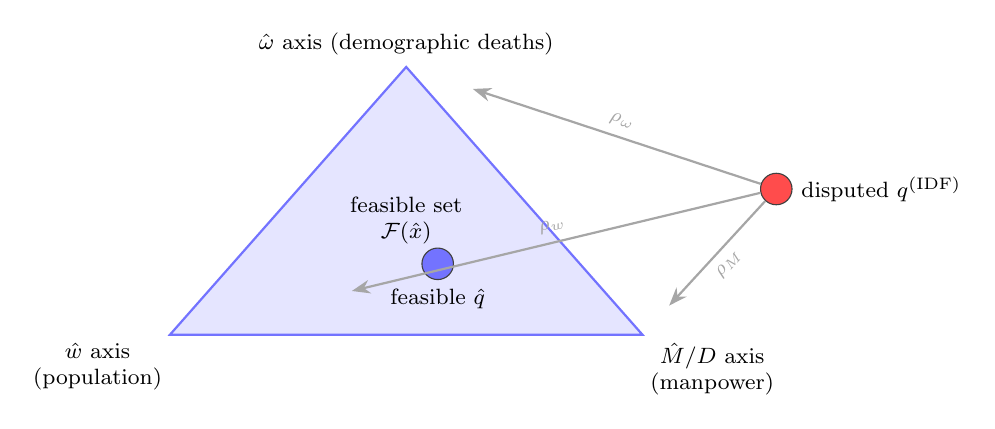
\begin{tikzpicture}[
  >=Stealth, font=\small,
  vert/.style={circle,draw=black!75,fill=white,inner sep=1.5pt,minimum size=4mm},
  feas/.style={fill=blue!10,draw=blue!55,thick},
  arr/.style={->,>=Stealth,gray!70,thick},
  lab/.style={font=\footnotesize,inner sep=2pt}
]
\coordinate (T)  at ( 0   , 2.5);
\coordinate (BL) at (-3.0 ,-0.9);
\coordinate (BR) at ( 3.0 ,-0.9);

\draw[feas] (T) -- (BL) -- (BR) -- cycle;
\node[lab,align=center] at (0,0.55) {feasible set\\$\mathcal F(\hat x)$};

\node[vert,fill=blue!55] (P) at (0.4, 0.0) {};
\node[lab,below=1pt of P] {feasible $\hat q$};

\node[vert,fill=red!70] (Q) at (4.7,0.95) {};
\node[lab,right=1pt of Q] {disputed $q^{(\mathrm{IDF})}$};

\draw[arr] (Q) -- ($(T)!0.18!(Q)$)  node[midway,above,sloped,font=\scriptsize] {$\rho_\omega$};
\draw[arr] (Q) -- ($(BR)!0.20!(Q)$) node[midway,below,sloped,font=\scriptsize] {$\rho_M$};
\draw[arr] (Q) -- ($(BL)!0.30!(Q)$) node[midway,above,sloped,font=\scriptsize] {$\rho_w$};

\node[lab] at (T)  [above=2pt] {$\hat\omega$ axis (demographic deaths)};
\node[lab] at (BL) [below left=1pt,align=center]  {$\hat w$ axis\\(population)};
\node[lab] at (BR) [below right=1pt,align=center] {$\hat M/D$ axis\\(manpower)};
\end{tikzpicture}
\caption{\textbf{Contradiction triangle (conceptual schematic).} The feasible set $\mathcal F$ is bounded by three independently measured ``axes''; the contradiction radius $\rho=\min(\rho_\omega,\rho_w,\rho_M)$ is the cheapest standardised revision of a single axis that carries a disputed claim into $\mathcal F$ (Definition~\ref{def:radius}). Each axis is owned by a different institution, which is what makes the relation under-fudgible: rescuing a claim on one axis leaves fingerprints on that axis's measurement.}
\label{fig:contradiction-triangle}
\end{figure}

\paragraph{Computation.} Each axis radius is available in closed form. On the demographic axis, inverting \eqref{eq:qmu} gives the composition a claim requires at exposure $\mu$, $\omega_{\mathrm{needed}}(q,\mu)=(1-q)\,\hat w/(\hat w+\mu(\hat a-\hat f))$; granting the claim the most favourable $\mu$ in the admissible range yields the interval of rationalising compositions $[\omega_{\mathrm{needed}}(q,\mu_{\mathrm{hi}}),\,\omega_{\mathrm{needed}}(q,\mu_{\mathrm{lo}})]$, and $\rho_\omega$ is the standardised distance from $\hat\omega$ to that interval (zero if $\hat\omega$ lies inside). The $w$ and $M$ axes are computed the same way through the identities $a'=1-w'$ and $f'=M'/\hat N$. This is the contradiction triangle of Figure~\ref{fig:contradiction-triangle}. In the Gaza application the last two axes cannot rescue the disputed claim at any remotely plausible magnitude (Section~\ref{sec:gaza}, Step~3 quantifies both), so $\rho=\rho_\omega$ there and radii are quoted in units of $\sigma_\omega$.

\paragraph{Diagnostic procedure.}
\begin{enumerate}[label=\textbf{D\arabic*.},leftmargin=*]
\item Fix the analysis window and total deaths $D$; carry the uncertainty in $D$ as a sensitivity dimension, not a constant.
\item Estimate $(w,a)$ from the population baseline and $\omega$ from identified-deaths records, checking each candidate $\omega$ source for selection mechanisms before use.
\item Calibrate the exposure range $[\mu_{\mathrm{lo}},\mu_{\mathrm{hi}}]$ from historical conflicts with known combatant status, and take an independent upper bound on $M$.
\item Compute $\mathcal F(\hat x)$ from \eqref{eq:feasible}.
\item For every disputed $\hat D_M^{(i)}$, report $q^{(i)}=\hat D_M^{(i)}/D$, the membership $q^{(i)}\in\mathcal F$, and $\rho^{(i)}$, under each anchor and each $D$ scenario.
\end{enumerate}
The test is symmetric: it scores ``too many combatants'' and ``zero combatants'' against the same set.

\section{Sensitivity bands under political bias}\label{sec:bias}

The bounds in Sections~\ref{sec:bounds}--\ref{sec:contradiction} treat each measured input as honest. We now allow the analyst to dial in distrust of specific sources. Political bias enters the confidence statement through Huber contamination: each source $i$ writes its likelihood as $(1-\varepsilon_i)L_i+\varepsilon_i Q_i$, with $Q_i$ adversarial in some class $\mathcal Q$ \citep{huber1964,huber1981,berger1986,gagnon2023}. The contamination parameter $\varepsilon_i\in[0,1]$ is the analyst's prior probability that source $i$ is producing a politically motivated reading rather than a measurement of the true distribution.

\begin{proposition}[Bias-robust sensitivity band]\label{prop:robust}
Let $\theta$ be a scalar estimand with $1-\alpha$ posterior credible interval $I_0=[L_0,U_0]$ under face-value sources, with the posterior supported on the identified set implied by the sources used. Suppose each source $i$ is independently contaminated with probability $\varepsilon_i$, and removing the sources in a set $T$ leaves an identified set of diameter $R_T$ (write $R_i:=R_{\{i\}}$).
\begin{enumerate}[label=(\roman*),leftmargin=*]
\item \emph{(Patternwise envelope.)} If the realised contamination pattern is $T$, every \emph{support-respecting} $1-\alpha$ credible interval---one whose endpoints lie in the posterior support, e.g.\ the equal-tailed or HPD interval---obtainable by adversarial replacement of the sources in $T$ lies within $[L_0-R_T,\ U_0+R_T]$. (An arbitrary credible interval can be widened without limit while retaining $1-\alpha$ coverage, so no finite envelope constrains that class.)
\item \emph{(Expected displacement.)} Averaging over the contamination pattern, the expected endpoint displacement is at most $\sum_i\varepsilon_i R_i$ plus higher-order terms in $\varepsilon$ involving the multi-removal diameters $R_T$, $|T|\ge 2$; when at most one source can be contaminated, the bound $\sum_i\varepsilon_i R_i$ is exact. The band
\begin{equation}\label{eq:Iepsilon}
I_\varepsilon \;=\; \Bigl[L_0-\textstyle\sum_i\varepsilon_i R_i,\; U_0+\textstyle\sum_i\varepsilon_i R_i\Bigr]
\end{equation}
is therefore a first-order sensitivity band for the interval endpoints---not a uniform envelope over realised contaminated intervals, whose endpoints can move by up to $R_T$ on the (probability $\le\varepsilon_i$) contamination events.
\item \emph{(Quantile displacement.)} If additionally the posterior mixture weight on contaminated components is at most $\tau:=1-\prod_i(1-\varepsilon_i)$---which holds when the component marginal likelihoods are comparable, and must otherwise be checked, since posterior weights are proportional to prior pattern probabilities \emph{times} component marginal likelihoods---and the face-value posterior density exceeds $m>0$ on the segment between the clean and contaminated $u$-quantiles, then
\[
\bigl|\hat Q_\varepsilon(u)-\hat Q_0(u)\bigr|
   \;\le\; m^{-1}\tau,
\qquad u\in\{\alpha/2,\,1-\alpha/2\}.
\]
\end{enumerate}
\end{proposition}
Proof in Appendix~\ref{app:proofs}.

\paragraph{Practice.} Set $\varepsilon_i\approx 0.05$ for widely-trusted demographic sources (Palestinian Central Bureau of Statistics, health-ministry demographic records consistent with independent surveys) and $\varepsilon_i\approx 1$ (i.e., adversarial) for belligerent claims; \eqref{eq:Iepsilon} then absorbs the assumed political bias automatically. We apply the band to the identified-set endpoints---the degenerate case in which the posterior is supported on the identified set and the credible interval is the set itself. In the Gaza application the removal diameters, each computed as the diameter of the exposure-agnostic identified set with that source removed and the remaining inputs held at their envelopes, are: $R_{\mathrm{demo}}=\nRDemo{}$ (dropping the demographic record leaves only the manpower bound $q\le M/D$); $R_{\mathrm{census}}=\nRCensus{}$ (letting $w$ range over a generous global envelope $[0.70,0.76]$, with $a=1-w$, gives the set $[0,\,q(1;w{=}0.76)]=[0,\nRCensusSet{}]$); and $R_M=\nRM{}$ (dropping the manpower source frees $f$ up to its logical cap $f\le a$, at which the set reaches the all-male ceiling $1-\omega$). The global envelope $[0.70,0.76]$ is a background constraint---a generous envelope for the demographic structure of young, high-fertility populations of the kind at issue here, justified independently of the census being removed---so it survives removal of the census source, and the removal diameter is computed under it. Then $\varepsilon=0.05$ inflates the exposure-agnostic upper bound by $0.05\,(\nRDemo{}+\nRCensus{}+\nRM{})\approx \nHuberPP{}$ percentage points---from $\nQOne{}\%$ to $\nHuberInflated{}\%$---which still rejects the upper end of the disputed claim.

\section{Application: Gaza 2023--2026}\label{sec:gaza}

We instantiate the framework using inputs measured by institutions other than the claimant, each cross-checkable against sources independent of the claim under test (the Gaza MoH sits within Gaza's governing structure, and its standing here rests on record rather than position: its register of named dead---the only full-coverage one, and the working basis for analysts on both sides---kept an age--sex composition that stood publicly uncontested for years while the total and the combatant status of the dead were disputed continuously; the composition is consistent with an independent household survey, and the opposing belligerent has since accepted the cumulative toll outright): Palestinian Central Bureau of Statistics (PCBS) population structure \citep{pcbs}; total deaths from the UN Office for the Coordination of Humanitarian Affairs (OCHA) and the Gaza Ministry of Health (MoH) \citep{ochaopt}; OHCHR and MoH demographic death records \citep{ohchr2024}; the Gaza Mortality Survey (GMS) household study \citep{spagatlgh2026}; excess-mortality information \citep{khatib2024,jamaluddine2025}; and combatant-strength estimates from the International Institute for Strategic Studies (IISS), the Royal United Services Institute (RUSI), and the Center for Strategic and International Studies (CSIS) \citep{iiss2024,rusi2024}. The IDF claim itself \citep{idfclaim} is the object of the test, not an input. All derived numbers in this section---every bound, radius, and generated table entry---are computed by a validation script in the companion repository, which emits them as the numeric macros and tables this text includes, recomputes each from the raw inputs, and fails on any internal discrepancy.

\begin{table}[ht]
\centering
\caption{\textbf{Diagnostic inputs for Gaza.} The disputed quantity $D_M$ is tested against the other rows. The adult-male class is males 18 and over, so $a=1-w$ exactly.}
\label{tab:gaza-inputs}
\begin{small}
\renewcommand{\arraystretch}{1.3}
\begin{tabularx}{\textwidth}{@{}>{\raggedright\arraybackslash}p{0.36\textwidth}>{\raggedright\arraybackslash}X>{\raggedright\arraybackslash}X@{}}
\toprule
Input & Value & Channel \\
\midrule
$w$ (women$+$children \emph{of population}) & $0.733$       & PCBS population structure \\
$a$ (males 18$+$ \emph{of population})      & $0.267$       & $=1-w$ \\
\addlinespace
$\omega$ (women$+$children \emph{of the dead}) & $0.560$ (MoH record; primary anchor) & identified deaths, consistent with GMS \\
          & $0.693$ (OHCHR verified sample)  & residential-strike stratum \\
\addlinespace
$D$ (direct deaths, late 2025) & $70$k (MoH) $/$ $\nDCorr{}$k (GMS-corrected) $/$ $\nDMax{}$k ($+$missing) & MoH, GMS, missing-persons registry \\
$f$ (combatant share of population) & $0.0157$--$0.0269$ ($0.020$ central) & Hamas / Palestinian Islamic Jihad pre-war manpower $/$ population \\
$\mu$ (exposure ratio) & grid $\{1,1.5,2,2.5,3.5,5\}$; historically calibrated $[2,3.5]$ & \citet{frost2026,cockerill2024} \\
$M$ (pre-war combatant stock) & $35{,}000$--$60{,}000$ (central $45{,}000$) & IISS / RUSI / CSIS \\
\midrule
claim (tested, not an input) & $17$--$25$k combatants killed & IDF public statements \\
\bottomrule
\end{tabularx}
\end{small}
\end{table}

\paragraph{Anchor choice.} The two demographic records of the dead measure different things. The OHCHR sample ($n=8{,}119$) applies a strict three-source verification rule under which $7{,}607$ of the $8{,}119$ verified deaths ($94\%$) occurred in residential buildings, where women and children predominate \citep{spagatcockerill2024}; it is best read as a stratum-specific measurement, not an estimate of the overall $\omega$. The MoH full record ($n\approx 70{,}000$) covers all recorded deaths, and its demographic composition has a track record no other input in this application can match: the record is a list of named individuals from which analysts on both sides worked throughout the war, and across years of dispute over its figures the contest was always about the total and about who among the dead was a combatant---never about the age--sex composition of the named list; the Israeli military has itself since accepted the MoH cumulative toll outright \citep{haaretzidf2026}. The composition is also consistent with the Gaza Mortality Survey, a household probability survey: the survey's women-children-and-elderly share ($56.2\%$) sits at the record's women-and-children share ($56.0\%$); the published survey tables do not provide the age--sex cross-tabulation needed for an exact match of the two estimands, so we read this as consistency rather than exact corroboration. The same survey estimates $75{,}200$ violent deaths against $49{,}090$ recorded over its window---the record captures roughly two-thirds of survey-estimated deaths \citep{spagatlgh2026}. We therefore anchor on the MoH record ($\omega=0.560$): a composition that stood publicly for years, uncontested in practice by either belligerent, earns its place by that history rather than by any institutional label. The figure comes from the record's three-category breakdown (children under 18: $32\%$; women 18$+$: $24\%$; men 18$+$: $44\%$), in which every person is classified by sex and adult status---elderly men sit inside the men-18$+$ class, matching the paper's $\mathrm{AM}$ definition exactly. The breakdown is that of the identified record as of early 2025, applied to the late-2025 cumulative toll; composition drift across 2025 is one of the systematic errors the conservative $\sigma_\omega$ allowance and the alternative anchors are there to absorb. The uncertainty scale we attach to it, $\sigma_\omega=0.01$, is a deliberately conservative systematic allowance---about five times the record's binomial standard error at $n\approx 70{,}000$---chosen so that radii quoted in $\sigma_\omega$ units \emph{understate} the discrepancy relative to pure sampling noise; every radius in this section scales inversely in this choice. We also report the OHCHR anchor---and a geometric blend of the two, a descriptive midpoint rather than an estimator---as sensitivities rather than blending them into a single aggregate. Because $\omega_{\mathrm{MoH}}<\omega_{\mathrm{OHCHR}}$, this choice is \emph{favourable} to high-combatant claims: every rejection below survives, a fortiori, under the alternative anchors.

The survey's representativeness has been contested: \citet{dellapergola2026} identify interviewer-level heterogeneity and protocol deviations and argue the population-level extrapolation is unreliable; \citet{spagatreply2026} respond that the conclusions survive excluding the contested teams (the violent-death estimate falls from $75{,}200$ to $59{,}200$ under maximal exclusion, with the demographic composition intact). For present purposes the dispute is instructive precisely because it does not touch the bounds. It concerns the \emph{level} of the death toll, an input our identified set does not use: $q(\mu)$ depends on $(\omega,w,a,f)$ only, and the demographic composition---the one quantity the framework takes from the survey---is stable across every specification in the exchange, including the critics' own exclusions and the extreme all-missing-dead scenario (the survey's women-children-elderly share of violent deaths moves from $56.2\%$ only to $52.2\%$; note this classification includes people over 64 and so is not identical to our $\omega$ class, but it is the composition measure the exchange contests). The undercount factor enters solely through the $D$-sensitivity dimension of Step~3 ($D=70$--$\nDMax{}$k), and only its upward corrections matter there. Downward revisions of the toll require no new scenario, because the direction of the challenge is self-defeating for the claim it might appear to assist: if the critics were right and the true toll were \emph{lower}, the claimed combatant counts would convert to \emph{higher} shares $q^{(i)}=\hat D_M^{(i)}/D$, moving the disputed claim further outside the feasible set while leaving the set itself unchanged. This is the under-fudgible structure at work: contesting one measurement re-routes, but does not relieve, the burden of the contradiction.

\paragraph{Step 1: rejecting uniform random violence.} The naive null ``violence is uniform across the population'' predicts $\E\,\omega=w=73.3\%$. Even the OHCHR sample ($\hat\omega=69.3\%$) sits $z=\nZUnif{}$ binomial units below it---a descriptive discrepancy measure, since the verified sample is selected rather than random (a formal test, if the sample were a probability sample, would reject overwhelmingly: one-sided $p\approx \nPUnif{}$)---and the MoH full record ($\hat\omega=56.0\%$) departs from uniformity by a far wider margin. Adult males are overrepresented among the dead---as they must be once any combatants die or civilian men carry any excess exposure. Rejecting uniformity is necessary but not sufficient to rationalise any \emph{specific} combatant share; the question is how the adult-male excess splits between the two explanations, and that is precisely what $\mu$ indexes.

\paragraph{Step 2: the identified set.} On the MoH anchor, Theorem~\ref{thm:bounds} gives
\[
q(1)=\nQOne{}\%,\qquad q(1.5)=\nQOnePointFive{}\%,\qquad q(2)=\nQTwo{}\%,\qquad q(\mu)\le 0\ \text{for}\ \mu\ge \nMuStarCeil{}
\]
(the root of $q(\mu)=0$ sits at $\mu^\ast\approx \nMuStar{}$). The exposure-agnostic set (any $\mu\ge 1$; the upper endpoint is $q(1)$ and the lower is clipped at zero) is $q\in[0,\,\nQOne{}\%]$; the historically calibrated set ($\mu\in[2,3.5]$, \citealp{frost2026}) is $q\in[0,\,\nQTwo{}\%]$. The manpower bound $M/D=\nMOverD{}$ never binds, and the manpower input matters little on the demographic side either: over the full institutional range $M\in[35{,}000,\,60{,}000]$ ($f\in[0.0157,0.0269]$), $q(1)$ moves only between $\nQOneFLo{}\%$ and $\nQOneFHi{}\%$; we use the central $f=0.020$ throughout. Table~\ref{tab:sensitivity} reports the full anchor$\times\mu$ grid; the OHCHR anchor caps $q$ at $\nQOneOhchr{}\%$ already at $\mu=1$, and at calibrated exposure it admits no combatant share at all---an empty set there means that stratum's composition, the calibrated range, and the model are jointly inconsistent, a diagnostic about extrapolating residential-strike composition conflict-wide rather than additional evidence against any claim.

\begin{table}[ht]
\centering
\caption{\textbf{Sensitivity of the identified-set upper endpoint.} Each cell is $q(\mu)=1-\omega\,(w+\mu(a-f))/w$ evaluated at $w=0.733$, $a=0.267$, $f=0.020$: the largest combatant share consistent with anchor $\omega$ if civilian adult men die at exactly $\mu$ times the per-capita rate of women and children. The identified set for exposure range $[\mu_{\mathrm{lo}},\mu_{\mathrm{hi}}]$ is $[q(\mu_{\mathrm{hi}}),\,q(\mu_{\mathrm{lo}})]\cap[0,1]$. Dashes: $q(\mu)\le 0$ at that exact exposure ratio, i.e.\ the anchor admits no positive combatant share there; an exposure \emph{range} whose lower end still gives $q\ge 0$ has its lower endpoint clipped at zero (zero combatants remains consistent), while a range lying entirely in the dashed region yields an empty set: that anchor and that exposure range are jointly inconsistent. Exposure ratios calibrated on historical conflicts are $\mu\gtrsim 2$ \citep{frost2026,cockerill2024}.}
\label{tab:sensitivity}
\begin{small}
\renewcommand{\arraystretch}{1.3}
\begin{tabular}{@{}lcccccc@{}}
\toprule
Anchor $\omega$ (share of dead) & $\mu{=}1$ & $\mu{=}1.5$ & $\mu{=}2$ & $\mu{=}2.5$ & $\mu{=}3.5$ & $\mu{=}5$ \\
\midrule
MoH (GMS-consistent), $\omega=0.560$ & 25.1\% & 15.7\% & 6.3\% & -- & -- & -- \\
Blend (geometric), $\omega=0.623$ & 16.7\% & 6.2\% & -- & -- & -- & -- \\
OHCHR (residential-strike stratum), $\omega=0.693$ & 7.3\% & -- & -- & -- & -- & -- \\
\bottomrule
\end{tabular}
\end{small}
\end{table}


\paragraph{Step 3: testing the IDF claim.} The claim's endpoints were briefed at different dates against different contemporaneous tolls ($17$k in 2024, $25$k in early 2026 alongside the ${\sim}70$k cumulative figure); we read $17$--$25$k as the claim's cumulative range and convert both endpoints over the same final denominator, which is the reading most favourable to the claim at its lower end. Over the MoH-confirmed denominator $D=70$k, the claimed $17$--$25$k combatants convert to $q^{\mathrm{IDF}}=\nIdfQLo{}\%$--$\nIdfQHi{}\%$, i.e.\ a civilian-to-combatant ratio of roughly $\nIdfCcrAtHi{}{:}1$--$\nIdfCcrAtLo{}{:}1$. The contradiction radius of Definition~\ref{def:radius}---which grants the claim the most favourable $\mu$ in the admissible range---splits cleanly across the two endpoints:
\begin{itemize}[leftmargin=*]
\item \emph{The $25$k endpoint is infeasible for any $\mu\ge 1$.} Rationalising $q=\nIdfQHi{}\%$ on the MoH anchor requires $\mu=\nMuIdfHi{}$: civilian adult men would have to die at less than half the per-capita rate of women and children, which no documented mechanism in this conflict supports. On the demographic axis the radius is $\rho_\omega\approx \nRhoOmegaAg{}$ units of $\sigma_\omega$ with agnostic exposure and $\approx \nRhoOmegaCal{}$ with calibrated exposure (and $\approx \nRhoOhchrAgRound{}$--$\nRhoOhchrCalRound{}$ on the OHCHR anchor). For the other two axes we attach the scales $\sigma_w=0.005$ (a generous allowance for census projection error) and $\sigma_M=12{,}500$ (the half-width of the institutional range for $M$, $[35\mathrm{k},60\mathrm{k}]$). Even granting $\mu=1$, rescuing $q=\nIdfQHi{}\%$ through the census alone requires $w'\approx \nWRescue{}$ rather than the measured $0.733$---$\rho_w\approx \nRhoW{}$ units of $\sigma_w$, a twelve-percentage-point census error---and rescuing it through the manpower channel ($f'=M'/\hat N$) requires a pre-war stock of ${\approx}\nMRescue{}$, eight times the IISS estimate: $\rho_M\approx \nRhoM{}$ units of $\sigma_M$. The minimum in Definition~\ref{def:radius} is therefore attained on the demographic axis, and $\rho=\rho_\omega$ throughout this section.
\item \emph{The $17$k endpoint is feasible only at the edge, and only without calibration.} At $q=\nIdfQLo{}\%$ the required exposure ratio is $\mu=\nMuIdfLo{}$: barely inside the mathematically admissible range, so $\rho=0$ on the MoH anchor only if civilian men in Gaza were essentially no more exposed than women and children. Any exposure differential beyond $\mu\approx \nMuIdfLo{}$ puts the claim outside the set; the historically calibrated range $\mu\in[2,3.5]$---obtained from historical Gaza conflicts where combatant status is recorded \citep{frost2026}---puts it $\rho_\omega\approx \nRhoIdfLoCal{}$ units of $\sigma_\omega$ outside. The lower endpoint is therefore feasible only marginally, resting on the single most claim-favourable value of the one parameter the data cannot pin down. And even that value buys only the bottom of the claimed range: $\mu=1$ caps the combatant share at $\nQOne{}\%$, roughly $\nQOneCount{}$k of the $70$k dead, so every count the IDF asserts above that---most of the $17$--$25$k interval---requires, \emph{on top of} $\mu=1$, moving the census $w$, the demographic record $\omega$, or the combatant stock $M$ as well (the cheapest manpower-only rescue already needs a stock more than three times the institutional estimate). Granting equal exposure is thus not enough to rationalise the claim; it only relocates the remaining burden onto quantities other institutions measure.
\end{itemize}
The rejection is robust to the denominator: the survey's ratio of estimated to recorded violent deaths ($75{,}200/49{,}090\approx \nGmsRatio{}$) scales the $70$k record to $D\approx \nDCorr{}$k, and adding the missing gives $D\approx \nDMax{}$k (treating the missing as additional assumes the survey estimate does not already include them, which is why both corrected scenarios are reported); these corrections lower $q^{\mathrm{IDF}}$ to $\nIdfQCorrLo{}$--$\nIdfQCorrHi{}\%$ and $\nIdfQMaxLo{}$--$\nIdfQMaxHi{}\%$ respectively, but the required exposure ratios ($\mu\le \nMuMaxSeventeen{}$ for $17$k, $\mu\le \nMuMaxTwentyFive{}$ for $25$k) remain below the calibrated range. (Applying the recorded $\omega$ to the corrected totals assumes the unrecorded dead share the recorded demographic mix, which the survey's demographic breakdown supports; extrapolating the survey-period ratio to the full record is itself an assumption, which is why the uncorrected $D=70$k is the primary test.) The correction also works against the claim on the civilian ledger, by arithmetic alone: the claimed combatant count is a fixed number, so every one of the ${\sim}\nCorrAdd{}$ deaths the correction adds (${\sim}\nCorrAddMissing{}$ with the missing) is a civilian death under the claim's own accounting. The combatant side cannot absorb the increment: $25$k dead combatants is already $\nKillFracTwentyFiveIiss{}\%$ of the IISS stock, and absorbing the correction as well would require $\nAbsorbNeeded{}$k, above even the $60$k top of the institutional range for $M$. The claim's implied civilian toll therefore rises from $\nCivMohLo{}$--$\nCivMohHi{}$k at $D=70$k to $\nCivCorrLo{}$--$\nCivCorrHi{}$k at $D=\nDCorr{}$k ($\nCivMaxLo{}$--$\nCivMaxHi{}$k at $D=\nDMax{}$k), and its implied civilian-to-combatant ratio worsens from roughly $\nIdfCcrAtHi{}{:}1$--$\nIdfCcrAtLo{}{:}1$ to $\nCcrCorrLo{}{:}1$--$\nCcrCorrHi{}{:}1$ ($\nCcrMaxLo{}{:}1$--$\nCcrMaxHi{}{:}1$). The undercount debate is thus asymmetric for the claimant: a smaller toll converts the claimed counts to shares the demographic record rejects outright, and a larger toll concedes tens of thousands of additional civilian dead. No denominator in the empirically supported range helps; making the claimed counts consistent with calibrated exposure would instead require $D\gtrsim \nDNeeded{}$k for the $17$k count and $D\gtrsim \nDNeededHi{}$k for $25$k---roughly four to six times the recorded toll. The first-order sensitivity band of Proposition~\ref{prop:robust}, with $\varepsilon=0.05$ on each core input and the removal diameters of Section~\ref{sec:bias}, inflates the exposure-agnostic upper endpoint from $\nQOne{}\%$ to $\nHuberInflated{}\%$---still below the claim's upper endpoint. (The patternwise worst case is starker but works in the same direction: if the demographic record itself is the contaminated source, the analysis reduces to the manpower bound $q\le \nMOverD{}$, which is exactly why the record's consistency with an independent household survey carries the weight it does.)

\paragraph{The adult-male death budget.} Figure~\ref{fig:gaza-budget} restates the test as an allocation problem. The demographic record fixes the composition of the $70{,}000$ confirmed dead: $\nBudgetWc{}$ women and children and $\nBudgetMen{}$ adult men. Every hypothesis about combatant deaths spends the same $\nBudgetMen{}$-person budget, splitting it between combatants and civilian men; the difference between hypotheses is only where the dividing line falls, and each position of the line implies a per-capita death rate for every class. Those implied rates are where the claim breaks. The women-and-children rate is pinned at $\nRateWc{}\%$ of their population. Random violence with no targeting at all would kill every class at $\nRateRandom{}\%$ and put combatant deaths at $\nRandomCombatants{}$ ($q=\nRandomQ{}\%$, inside the calibrated set); the record sits far from that composition (Step~1), so the observed male excess needs explaining, but random slaughter alone already generates combatant tolls of the order the spatial model finds. The IDF claim sits at the opposite pole. At $17$k it implies $\nKillFracSeventeenIiss{}\%$ of the IISS combatant stock killed (we use the $45{,}000$ point estimate throughout---the central institutional figure, and more favourable to the claim than the IDF's own pre-war figure of $30{,}000$, on which the kill fraction is $\nKillFracSeventeenIdf{}\%$; even at the top of the institutional range, $60{,}000$, the $17$k claim still kills $\nKillFracSeventeenTop{}\%$ of the force) while civilian men die at $\nRateAmcivSeventeen{}\%$, barely above the women-and-children rate ($\mu=\nMuIdfLo{}$). At $25$k it implies $\nKillFracTwentyFiveIiss{}\%$ of the stock killed ($\nKillFracTwentyFiveIdf{}\%$ on the IDF's own figure) while civilian men die at $\nRateAmcivTwentyFive{}\%$, less than half the women-and-children rate ($\mu=\nMuIdfHi{}$). The claimed campaign would have to be selective enough to kill combatants at $\nSelSeventeen{}$ to $\nSelTwentyFive{}$ times the per-capita rate of civilian men in the same population, yet indiscriminate enough that those same civilian men gain no more exposure than women and children. Both rates are arithmetically forced by the allocation; what the budget exposes is their conjunction---a campaign at once maximally selective across the combatant line and exposure-blind on the civilian side of it. Even the limiting concession, counting all $\nBudgetMen{}$ dead men as combatants, caps $q$ at $\nAllMenQ{}\%$ and---under the exposure model---requires a combatant stock of $\nAllMenStock{}$, the entire adult-male population: with $\mu\ge 1$ and any positive civilian death rate, a non-empty civilian-male class must produce civilian-male deaths, so zero civilian men among the dead forces the civilian-male class itself to be empty (raw bookkeeping alone would require only the $\nBudgetMen{}$). That stock is twenty times the IDF's own estimate; and since the claim itself stops at $25$k, it concedes $\nConcedeLo{}$--$\nConcedeHi{}$ of the dead men as civilians while still demanding the rates above.

\begin{figure}[!tp]
\centering
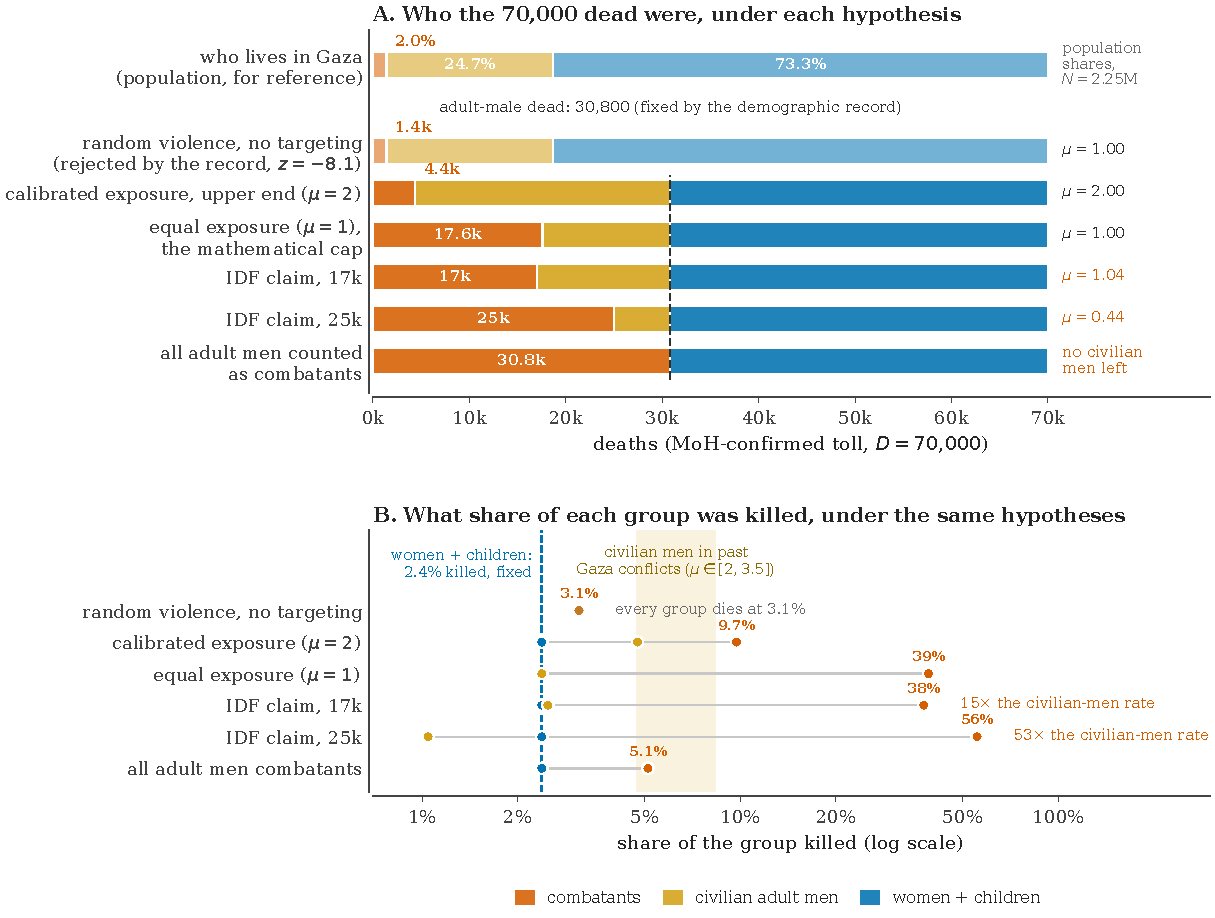
\includegraphics[width=\textwidth]{fig_gaza_budget}
\caption{\textbf{The adult-male death budget.}
\textbf{(A)} The two lighter bars are references. The top bar is the population: $2.25$M people, $2.0\%$ combatants, $\nShareAmCiv{}\%$ civilian adult men, $73.3\%$ women and children. The second is random violence with no targeting, under which the dead mirror the population ($\nRandomCombatants{}$ combatants); the record's composition lies far from it (even the verified OHCHR sample sits $z=\nZUnif{}$ binomial units below; Step~1). The four full-colour rows are hypotheses about combatant deaths, and all divide the same $\nBudgetMen{}$ dead adult men fixed by the MoH demographic record ($\omega=0.560$; dashed line) between combatants (rust, count printed) and civilian adult men (gold). The right margin gives the exposure ratio $\mu$ each split implies. The record's uncertainty ($\sigma_\omega=0.01$) moves the $\nBudgetMen{}$ line by about $\pm \nBudgetShift{}$, invisible at this scale.
\textbf{(B)} The same rows, converted to the share of each group killed (log scale), with population denominators $\nPopWc{}$ women and children, $\nPopAmCiv{}$ civilian men, and $45{,}000$ combatants (the central institutional estimate; more favourable to the claim than the IDF's own pre-war figure of $30{,}000$, though a larger stock would lower the kill fractions further; percentages printed at the combatant dots). The women-and-children share is fixed at $\nRateWc{}\%$; the shaded band is where civilian men fall at the exposure ratios measured in past Gaza conflicts, $\mu\in[2,3.5]$ \citep{frost2026}. The IDF rows require combatants to die at $\nSelSeventeen{}\times$ ($17$k) and $\nSelTwentyFive{}\times$ ($25$k) the rate of civilian men, while those civilian men die at or below the women-and-children rate; on the IDF's own pre-war stock of $30{,}000$ the claim implies $\nKillFracSeventeenIdf{}$--$\nKillFracTwentyFiveIdf{}\%$ of the force killed. The bottom row counts every dead man as a combatant: it caps $q$ at $\nAllMenQ{}\%$ and needs a combatant stock of $\nAllMenStock{}$, twenty times the IDF's estimate. All values are computed by the validation script from the inputs of Table~\ref{tab:gaza-inputs}.}
\label{fig:gaza-budget}
\end{figure}

\paragraph{Step 4: the named-combatant cross-check.} A joint investigation by \emph{The Guardian}, +972 Magazine, and Local Call \citep{guardian972db2025} reported that the Israeli Military Intelligence directorate's internal database listed $8{,}900$ named Hamas and Palestinian Islamic Jihad operatives dead or probably dead as of May 2025, against a contemporaneous recorded toll of ${\sim}53{,}000$: $q\approx \nAmanQ{}\%$, inside the exposure-agnostic identified set and far below the public claim of the same period. We treat this as corroborating, not primary, evidence---the database's coverage and classification rules are not public---but it is notable that the belligerent's own accounting apparatus lands inside the bound its public statements violate. The database also completes a chain drawn entirely from the claimant's own published figures. The IDF's pre-war estimate of the force it faced is $30{,}000$; its public claim of $17$--$25$k killed therefore asserts that $\nKillFracSeventeenIdf{}$--$\nKillFracTwentyFiveIdf{}\%$ of that force is dead. Converting the same claim over the ${\sim}70$k cumulative toll the IDF has itself accepted gives $q=\nIdfQLo{}$--$\nIdfQHi{}\%$---at the edge of the exposure-agnostic cap of $\nQOne{}\%$ at one end and past it at the other---while its own intelligence accounting, as above, sits at $\nAmanQ{}\%$. Stock, kill claim, accepted toll, and internal database are all the claimant's numbers. The first three are already mutually strained before a single external measurement enters---$\nKillFracSeventeenIdf{}$--$\nKillFracTwentyFiveIdf{}\%$ of the stated force killed, with conversions at or past the feasibility cap---while the database, whatever its coverage, shows the claimant's own accounting apparatus operating far below its public claim without contradicting it outright. The demographic record sharpens the tension; it does not create it.

\paragraph{The manpower ledger.} The claim's coherence can also be audited entirely within the belligerent's own accounting, using no Palestinian-measured input at all. This audit does not move the bounds; it prices the remaining escape route. The IDF's official pre-war estimate of Hamas strength is $30{,}000$ fighters in 24 battalions \citep{jpostbattalions2024}. Its assessment after the October 2025 ceasefire is that more than $22{,}000$ operatives were killed---and that the military wing nevertheless fields roughly $20{,}000$ operatives today \citep{iticledger2026}. These figures are jointly consistent only if at least $\nLedgerRecruits{}$ operatives were recruited during the war and the ceasefire, before counting the wounded and the detained; United States intelligence reported recruitment on exactly this scale ($10$--$15$k by January 2025, roughly matching losses over the same period; \citealp{reutersrecruit2025}). The ledger does not say where the recruits sit, but both placements concede ground. If they are among the dead, the killed-operatives count includes people who were civilians when the pre-war stock was measured, so the count stops being an answer to the question the public claim poses---how much of the force that existed on 7~October was destroyed. If they are among the living, the killed may all be pre-war stock, but the claimant then asserts wartime recruitment of at least $\nLedgerRecruits{}$ against the more than $22{,}000$ it counts killed---recruitment replacing over half its claimed attrition, the wartime-recruitment concession of Section~\ref{sec:discussion}, made by its own assessment rather than by its critics. Either way, rescuing the claim on the manpower axis costs exactly what the framework says it must.

\paragraph{Step 5: convergence of methods.} Table~\ref{tab:convergence} is the central empirical exhibit. Methods with different data, assumptions, and failure modes---the identified set of this paper, demographic decompositions \citep{cockerill2024,frost2026}, the military's internal database, and a fully specified spatial Bayesian model (Appendix~\ref{app:spatial})---all lie within $q\in[0,{\sim}\nQOneCeil{}\%]$, with point estimates and calibrated bounds concentrated at the low end: in civilian-to-combatant terms, even the loosest bound concedes ${\sim}\nCcrAtQOne{}{:}1$, while the calibrated bounds and model-based estimates imply $\nCcrCalibratedFloor{}{:}1$--$\nSpatialCcr{}{:}1$ on direct deaths. The upper end of the public claim ($q=\nIdfQHi{}\%$) lies outside every method's range; the lower end ($q=\nIdfQLo{}\%$) is reached only at endpoints that grant civilian men no or minimal excess exposure---the $\mu\ge 1$ edge of the identified set and the top of the decomposition range---and lies above every calibrated bound and point estimate. The spatial model, whose priors and structure are documented in Appendix~\ref{app:spatial}, posterior-concentrates at $q=\nSpatialQ{}\%$ ($95\%$ credible interval $[\nSpatialQLo{}\%,\nSpatialQHi{}\%]$, civilian-to-combatant ratio $\nSpatialCcr{}{:}1$ $[\nSpatialCcrLo{},\nSpatialCcrHi{}]$); we report it as one model-based point within the identified set, not as the headline, because its position within the set is prior-sensitive in ways the bounds are not. Figure~\ref{fig:gaza-diagnostic} shows the identified-set geometry on the $(\omega,w)$ plane alongside the spatial posterior.

\begin{table}[ht]
\centering
\caption{\textbf{Convergence of methods on the Gaza combatant share.} Every method's range lies within $q\in[0,{\sim}26\%]$, with point estimates and calibrated bounds concentrated at the low end (the point estimates and calibrated bounds correspond to civilian-to-combatant ratios of roughly $3{:}1$ to $45{:}1$ on direct deaths). The upper end of the IDF claim ($35.7\%$) lies above every range; its lower end ($24.3\%$) is reached only at endpoints that grant civilian men no or minimal excess exposure (the $\mu\ge 1$ edge of the identified set, the top of the decomposition range) and lies above every calibrated bound and point estimate. The methods share some inputs (MoH record, PCBS census) and are convergent cross-checks, not statistically independent replicates.}
\label{tab:convergence}
\begin{footnotesize}
\renewcommand{\arraystretch}{1.3}
\begin{tabularx}{\textwidth}{@{}>{\raggedright\arraybackslash}Xll>{\raggedright\arraybackslash}X@{}}
\toprule
Method & Source & Implied $q$ & Note \\
\midrule
IDF public claim (17--25k of 70k) & \citep{idfclaim} & 24.3--35.7\% & object of the test \\
\midrule
Identified set, MoH anchor, $\mu\ge 1$ & this paper & 0.0--25.1\% & weakest assumption ($\mu\ge 1$) \\
Identified set, MoH anchor, $\mu\in[2,3.5]$ & this paper & 0.0--6.3\% & Frost-calibrated exposure \\
Aman named-militant database & \citep{guardian972db2025} & 16.8\% & named fraction: 8,900 of 53,000 (May 2025); coverage unknown \\
Male-bias model, MoH record & \citep{frost2026} & 11.1--16.9\% & B'tselem-calibrated \\
Demographic decomposition & \citep{cockerill2024} & 9.4--26.3\% & range of male-bias assumptions \\
Spatial Bayesian posterior & this paper, App.~\ref{app:spatial} & 1.5--3.0\% & prior-dependent; one point in the set \\
\bottomrule
\end{tabularx}
\end{footnotesize}
\end{table}


\begin{figure}[!tp]
\centering
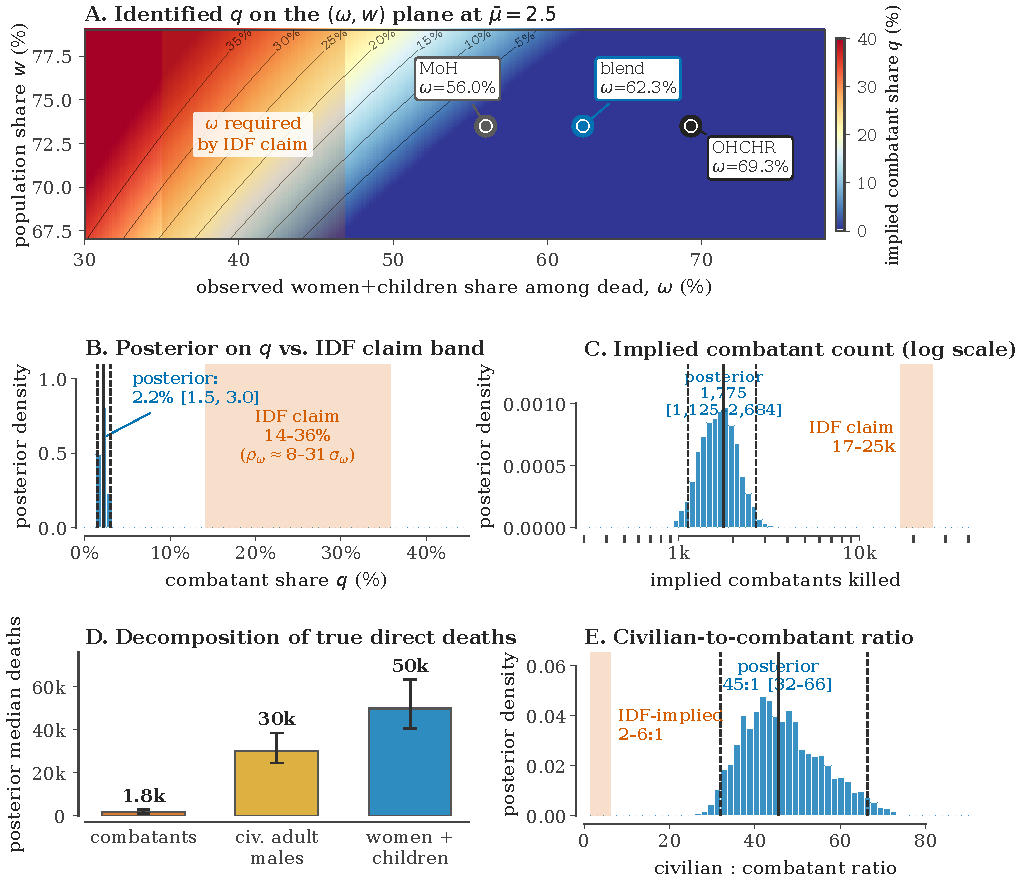
\includegraphics[width=\textwidth]{fig_gaza_diagnostic}
\caption{\textbf{The diagnostic for Gaza (2023--2026).}
\textbf{(A)} Identified $q$ on the $(\omega,w)$ plane at $\mu=2.5$ (values with $q(\mu)\le 0$ are shown clipped to zero: at exactly this exposure ratio such anchors admit no positive combatant share). Iso-$q$ contours are black; the OHCHR, blended, and Gaza Ministry of Health (MoH) anchors all sit in the low-$q$ (blue) region; the IDF claim requires $\omega$ in the red band on the far left, far from any observed anchor.
\textbf{(B)} Histogram of the spatial posterior on $q$ (median, 95\% credible interval as solid$+$dashed lines) vs.\ the IDF claim band converted to $q$; because the posterior's denominator is \emph{true} direct deaths, the band spans the denominator scenarios of the text ($D=70$k--$\nDMax{}$k), giving the claim its most favourable conversion at the low end.
\textbf{(C)} Implied combatants killed (log axis) vs.\ the IDF claim of $17$--$25$k.
\textbf{(D)} Posterior decomposition of true direct deaths under the spatial model (median ${\sim}82$k; the MoH-recorded ${\sim}70$k is the recovery-factor multiple of this): ${\sim}1$--$3$k combatants, ${\sim}30$k civilian adult men, ${\sim}50$k women and children.
\textbf{(E)} Civilian-to-combatant ratio: spatial-model posterior median $\nSpatialCcr{}{:}1$ vs.\ the IDF-implied band ($\approx \nIdfCcrAtHi{}{:}1$ on the MoH-confirmed denominator, up to $\approx \nCcrMaxHi{}{:}1$ under the largest denominator scenario). Panels B--E display the spatial model of Appendix~\ref{app:spatial}; the paper's headline claims rest on panels A and Table~\ref{tab:convergence}, not on the posterior.}
\label{fig:gaza-diagnostic}
\end{figure}

\paragraph{Symmetry.} The same machinery tests the polar narrative $q=0$ (``all the dead are civilians''). On the MoH anchor, $q=0$ requires $\mu=\nMuStar{}$---inside the calibrated range---so the demographic axis alone cannot reject it; the arithmetic is compatible with a purely civilian death toll if civilian men were about $\nMuStarOneDp{}$ times as exposed. What rejects $q=0$ is the named-combatant evidence: thousands of individually named militant dead are documented in the military's own database \citep{guardian972db2025}. The diagnostic thus does exactly what it should: it rejects the high claim on demographic grounds, rejects the zero claim on documentary grounds, and reports which axis does the work in each case.

\section{Empirical overview: 81 conflicts, 1899--2026}\label{sec:empirical}

The contradiction-radius diagnostic requires demographic micro-data and manpower estimates, and cannot be applied sharply to every historical conflict. The 81-conflict dataset is used here only to map where civilian-share uncertainty is large, where indirect mortality dominates, and which conflicts would benefit most from identified-deaths samples; the supplementary material provides a single master table detailing the bounds, binding relations, and confidence grades for all 81 conflicts, along with a complete list of primary sources used for each.

\begin{figure}[!tp]
\centering
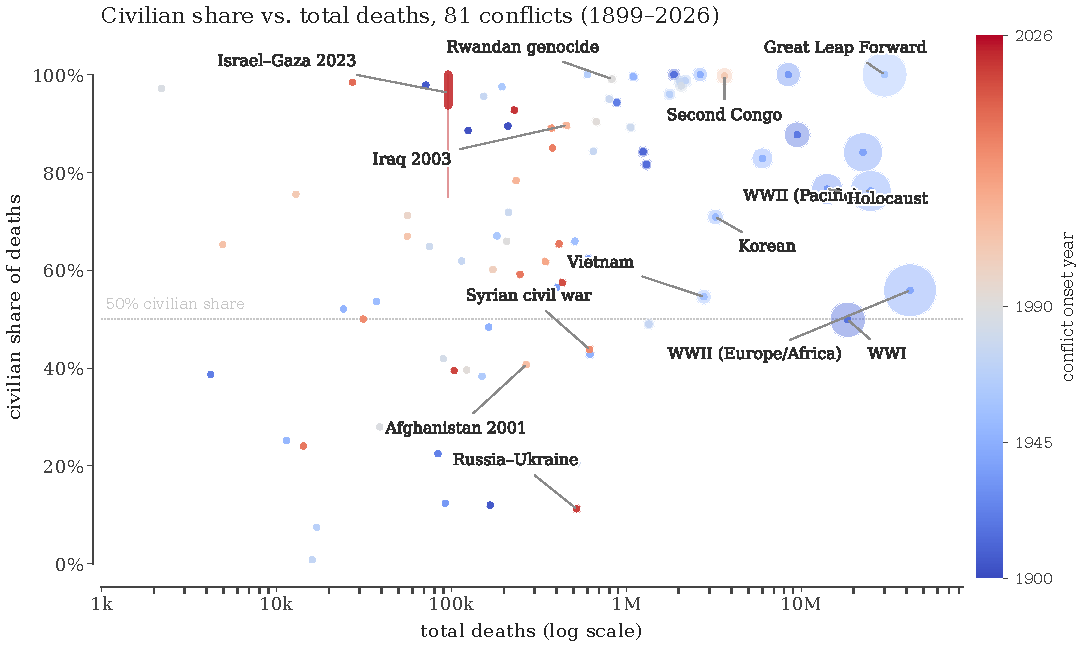
\includegraphics[width=0.95\textwidth]{fig_range_frame_civshare}
\caption{\textbf{Civilian share vs scale, 1899--2026.} Markers are conflicts; area increases with midpoint total deaths (min--max scaled, with a floor that keeps the smallest conflicts visible). Where sources state no ceiling for one casualty class, the class is bounded by the curated per-conflict totals or by the grand-total residual rather than treated as zero (Supplementary Material, \emph{How to read the tables}). Descriptively, the conflicts separate into two groups: combat-dominated interstate wars (civilian share $\lesssim 30\%$) and civilian-targeting events, famines, and atrocities (civilian share $\gtrsim 90\%$)---a mix of structurally different event types rather than a tested statistical bimodality.}
\label{fig:range-frame}
\end{figure}

\begin{figure}[!tp]
\centering
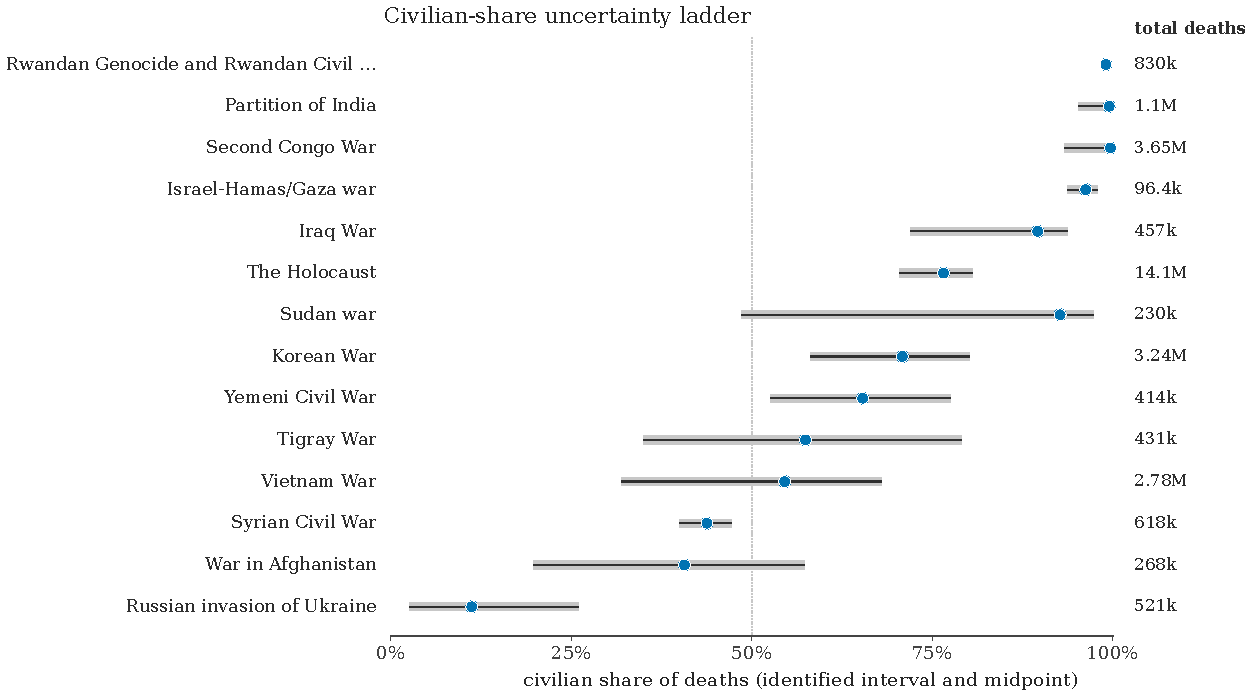
\includegraphics[width=0.92\textwidth]{fig_uncertainty_ladder}
\caption{\textbf{Civilian-share uncertainty ladder.} Selected high-leverage conflicts. Grey segments are the identified civilian-share interval; blue dots are the midpoints. Wide intervals mark conflicts where the next technical advance is a better identified-deaths sample, not a better plot.}
\label{fig:uncertainty-ladder}
\end{figure}

\paragraph{Generalisation.} The diagnostic transfers to any conflict with (i) a population demographic decomposition, (ii) an independent demographic survey of the dead, (iii) an independent manpower estimate at $t_0$, and (iv) a reported aggregate death total. Such inputs exist for Tigray 2020--2022 (Ethiopian Statistical Service plus WHO surveys), Syria 2011-- (Violations Documentation Center plus Syrian Network for Human Rights), the Mexican drug war (INEGI, the national statistics institute, plus CSIS/IISS cartel estimates), the Iraq War 2003--2011 \citep{burnham2006}, and Yemen 2014-- (Yemen Data Project plus the Armed Conflict Location and Event Data project, \citealp{acled}). Where these data are missing, the supplement marks the gap rather than inventing a contradiction radius.

\section{Discussion}\label{sec:discussion}

\paragraph{What the paper claims, and what it does not.} The conceptual contribution is the contradiction triangle (Theorem~\ref{thm:contradiction}): no single input can be moved far enough to rescue an infeasible claim without the move itself being visible against that input's independent measurement, and the contradiction radius $\rho$ gives a unit-free measure of how far a claim sits from the feasible set $\mathcal F$. Whereas \citet{spagat2009} frame war-death estimation as an \emph{arena of contestation}, our framework gives the analyst a numerical referee for that arena, in the spirit of \citet{lumpricebanks2013} for multiple systems estimation and \citet{radford2023} for Bayesian source aggregation. In the Gaza application the referee's ruling is deliberately modest: the data bound the combatant share of direct deaths at $\nQOneRound{}\%$ under only the minimal exposure assumption $\mu\ge 1$ and at about $\nQTwoRound{}\%$ under historically calibrated exposure, and the public claim of $\nIdfQLoRound{}$--$\nIdfQHiRound{}\%$ is rejected under every anchor and every calibrated exposure assumption we examined---its upper endpoint is arithmetically infeasible for any $\mu\ge 1$, and its lower endpoint survives only by asserting that civilian men were no more exposed than women and children ($\mu\approx 1$), against the calibration evidence---and much of the tension is internal, since the claimant's own pre-war stock estimate, the toll it accepts, and its intelligence database already contradict its public claim before any external measurement is consulted. The paper does \emph{not} claim that the spatial model's $q=\nSpatialQ{}\%$ is the truth; that number is one prior-dependent point inside the set, reported with its full model documentation so that readers can locate exactly which assumptions produce it.

\paragraph{Where the power comes from.} It is worth being explicit about why the bound binds. The demographic relation has one free behavioural parameter, the exposure ratio $\mu$, and the data pin the product, not the factors: a given deficit of women and children among the dead can be explained by combatants dying, by civilian men being more exposed, or by a mixture. High-combatant claims must therefore assert that $\mu\approx 1$---that civilian men in an urban war were no more exposed than women and children---at the same time as independent calibrations on conflicts with recorded combatant status put $\mu$ at $2$ or higher \citep{frost2026,cockerill2024}. The claim is not rejected by any single measurement but by the joint configuration; that is the under-fudgibility mechanism doing its work, and it is also why the diagnostic is hard to game: an actor wishing to defeat it must either assert a large, visible error at a single institution or coordinate distortions across a census bureau, a health ministry's death records, foreign military-balance assessments, and historical calibration data that predate the conflict.

The same structure prices the common defences of the claim. Each rescues feasibility on one axis by conceding ground elsewhere: large wartime recruitment relaxes the manpower constraint, but concedes that the war generates fighters faster than it removes them; differential undercounting of combatant deaths in the MoH record relaxes the demographic constraint, but concedes that the headline death toll is too low; a much larger true toll relaxes the arithmetic, but concedes a war more lethal than the claim's proponents otherwise allow. The framework does not adjudicate among these defences; it computes what each costs in standardised units of the input it moves (Section~\ref{sec:contradiction}) and forces the trade-off into the open.

\paragraph{Relation to convergent evidence.} The convergence table (Table~\ref{tab:convergence}) is, to our knowledge, the first side-by-side placement of the demographic-decomposition literature, the named-combatant documentary record, and a generative spatial model on the same scale. We read the residual disagreement---roughly $q\in[\nSpatialQRound{}\%,\nQOneCeil{}\%]$---as an honest statement of what current public data cannot resolve: it is essentially the width of the exposure-calibration question plus the classification question (who counts as a combatant, on which the named-list evidence and demographic methods can legitimately differ). Narrowing it further requires either a defensible conflict-specific measurement of $\mu$ or transparent, auditable combatant lists, not another aggregation rule.

\paragraph{Limitations.}
\begin{enumerate}[leftmargin=*]
\item Class $\mathrm{AM}$ is treated as a single bucket; finer age partitions (18--29, 30--49, 50$+$) tighten the bounds when age-resolved data exist, and the calibration of $\mu$ from near-cutoff age bands \citep{frost2026} is itself subject to sampling noise in small historical samples.
\item The exposure range $[\mu_{\mathrm{lo}},\mu_{\mathrm{hi}}]$ is imported from historical calibration; if the present conflict's exposure structure is genuinely outside that range, only the exposure-agnostic bound and the manpower bound survive. We report both throughout for this reason.
\item The radius standardises by a stated uncertainty scale (in the application, a conservative multiple of the sampling error); systematic error in an anchor (e.g.\ selection in who gets recorded as dead) is addressed by re-computing under alternative anchors, not by the radius itself. Section~\ref{sec:gaza} therefore reports all anchors, with the most claim-favourable one as primary.
\item The radius makes no probabilistic claim about how likely a given number of standardised units is; where a defensible sampling distribution exists, a bootstrap or non-parametric posterior is preferred for small demographic samples.
\item Combatant status is a legal-institutional category, not a demographic one. The framework bounds the share of deaths attributable to members of armed groups as counted by manpower estimates; disputes about who should count as a combatant move $M$ and the interpretation of named lists, and enter the diagnostic through those channels.
\item The estimand is the combatant share of \emph{direct} deaths throughout; indirect deaths from blockade, famine, or healthcare collapse require separate excess-mortality methodology \citep{checchiroberts2008,burnham2006,degommeguhasapir2010,gomez2025} and are outside the frame. The denominator scenarios varied in Section~\ref{sec:gaza} (survey-corrected and missing-persons totals) are corrections to the count of \emph{direct} deaths, so they change $D$ without changing the estimand.
\item The combatant stock $M$ and population shares $(w,a,f)$ are treated as fixed over the analysis window: wartime recruitment, ageing into the adult-male class, and displacement out of the territory are not modelled. Recruitment is the quantitatively relevant channel and is priced explicitly by the manpower ledger of Section~\ref{sec:gaza}; the demographic drifts are plausibly second-order at this window length.
\end{enumerate}

\paragraph{Reproducibility.} All bounds, radii, and derived table entries in this paper are computed by validation scripts that recompute them from the raw inputs, emit the numeric macros and tables the text includes, and fail on any internal discrepancy. In addition, the algebraic core of the framework (Appendix~\ref{app:proofs}) is formalised and machine-checked in Lean~4 with mathlib, and the remaining results are checked symbolically and exercised numerically by dedicated scripts. Code, the formal proofs, the spatial simulator, and all inputs are available in the companion repository.


\bibliography{../../content/refs}

\end{document}
